
\chapter{Running the Grover Search Algorithm}

This chapter will describe the experimental implementation of the so-called {\it Grover search algorithm} with our two-qubit quantum processor. The first section will provide a short introduction of the algorithm and motivate the interest in realizing it. The following sections will then discuss the details of the experimental realization of this algorithm. We will discuss the results that we obtained and compare the algorithm fidelity and runtime to that of an equivalent, classical algorithm. Finally, we will analyze all relevant errors made in our experiment.

\section{Introduction \& Motivation}

Search algorithms are of great importance in many domains of mathematics and computer science. One such search problem that often arises and which will be discussed in the following sections can be formulated in simple terms as follows:

\begin{theorem}
Assume that we have a search space $\begin{mathcal}S\end{mathcal}$ that consists of a finite number $N$ of states $s \in \begin{mathcal}S\end{mathcal}$. The solution to our search problem corresponds to a subset of $M$ states of the search space $\begin{mathcal}T\end{mathcal} \subset \begin{mathcal}S\end{mathcal}$. We can then define a search function $\Or(s):\begin{mathcal}S\end{mathcal}\to \{0,1\}$ that discriminates between states that solve the search problem and states that don't, such that $\Or(s) = 1$ for $s \in \begin{mathcal}T\end{mathcal}$ and $\Or(s) = 0$ otherwise.
\end{theorem}

Using this definition of the search problem, the goal of a search algorithm is to find all states $t\in\begin{mathcal}S\end{mathcal}$ for which $\Or(t) = 1$. In the following sections, for the sake of simplicity we will assume in the following sections that the solution set $\begin{mathcal}T\end{mathcal}$ contains only one single state $t$. This special case can easily be generalized to cases where more than one solution exists to the search problem.

\smallskip

The first step in order to solve a search problem of the kind described above is to map the problem above to a form suitable for solution by a digital (quantum) computer. For this, we first number and encode the $N$ input states $s_i \in \begin{mathcal}S\end{mathcal}$ in binary form such that $s_i = \sum\limits_{j=0}^l s_{ij}2^j $, where $l$ is the minimum required length of a binary register that can hold all $N$ input states. With this definition, it is then also trivial to reformulate $\Or$ such that the function operates on a binary input register instead of the original input states. 

\smallskip

Using these assumptions and definitions, it can then be shown that the most efficient classical search algorithm for solving the search problem above will use $\begin{mathcal}O\end{mathcal}(N)$ calls of the function $\Or$ to find the solution $t$ of the search problem. Assuming that the time to evaluate the function $\Or$ is far superior to the time needed to perform any other operation during the search algorithm, the number of calls to $\Or$ also corresponds approximately to the runtime of the whole search algorithm.

\smallskip

Amazingly, in 1997, Lev Grover found a quantum algorithm that could solve exactly the same search problem with only $\begin{mathcal}O\end{mathcal}(\sqrt{N})$ calls to the function $\Or$ \citep{Grover_Quantum_1997}. His algorithm achieves this by repeatedly calling a quantum-mechanical implementation of the function $\Or$ with a highly superposed qubit state and applying a special operator to the output state afterwards. The individual steps of the algorithm are straightforward and are given as follows:

\begin{enumerate}
 \item Initialize a qubit register to the state $\ket{\psi} = \ket{0}$ (corresponding to a binary input state $\ket{0000\hdots0_B}$)
 \item Apply the generalized Hadamard operation to the qubit register, producing a fully superposed quantum state $$\ket{\psi} = \frac{1}{\sqrt{N}}\sum\limits_{i=0}^{N-1} \ket{i}$$
 \item Repeat the following sequence $\begin{mathcal}O\end{mathcal}(\sqrt{N})$ times:
 \subitem a) Apply the {\it Oracle operator} $\ket{i}\to (-1)^{\Or(i)}\ket{i}$ to the state $\ket{\psi}$
 \subitem b) Apply the {\it diffusion operator} $\ket{i} \to -\ket{i}+\frac{2}{N}\sum\limits_{i=0}^{N-1}\ket{j}$ to the state $\ket{\psi}$
	\item Measure the state of the quantum register
\end{enumerate}

Here, we have enumerated the states of the qubit register from $\ket{0}$ to $\ket{N-1}$. Basically, the Grover algorithm makes use of quantum parallelism to solve the search problem $\begin{mathcal}O\end{mathcal}(\sqrt{N})$ times faster than the most efficient classical algorithm. To understand better its strategy used to solve the search problem, the different steps of the algorithm can be rephrased in the following, more intuitive way:

\begin{itemize}
\item First, it creates a fully superposed quantum state which contains all possible solutions to the search problem at once. The amplitudes and phases of each individual state are all equal in the beginning.
\item Then, it applies the so-called Oracle operator to this superposed state. The effect of the Oracle is to turn the phase of the states $t$ for which $\Or(t)=1$ by an angle $\pi$. As will be shown later, such an Oracle operator can be implemented in a straightforward way for any classical search function.
\item In the next step, it applies a diffusion operator to the quantum state which transfers a fraction of the amplitude from states with zero phase to the turned states, increasing thus the amplitude of the latter. In this process, the phases of all states also get turned back to zero, allowing the algorithm to repeat the sequence above.
\item Repeating these two operations increases the amplitude of the states that correspond to a solution of the search problem until the amplitudes of all the other states are zero. After that point, the process reverses and the amplitude is transferred back to the original states. It is therefore crucial to stop the repetition sequence given above after the right number of iterations.
\end{itemize}

By implementing the search function as a quantum operator, the Grover algorithm is able to evaluate it in one single call for all possible input states. This so-called {\it quantum parallelism} provides the basis for the speed-up of the search in comparision to a classical algorithm. However, being able to encode the result of the search function in the phase of a multi-qubit state does not directly translate to a speed advantage since it is usually very hard to extract this phase information from the quantum state. Indeed, to extract the values of all phases from an $N$-qubit state, it is necessary to perform $\begin{mathcal}O(2^N)\end{mathcal}$ measurements on an ensemble of identically prepared quantum states. However, extracting the state amplitudes from such a state takes only $\begin{mathcal}O\end{mathcal}(N)$ measurements, which in addition can usually be carried out in parallel. It is for this that the Grover algorithm uses an operator that transforms the information encoded in the phases of the qubits to an information encoded in their amplitude. However, since the conversion between phase to amplitude information through the application of an unitary operator is limited by certain physical constraints, the algorithm needs to repeat the encode-and-transfer sequence described above $\begin{mathcal}O(\sqrt{N})\end{mathcal}$ times. 

\smallskip

To analyze further the constraints and principles of the algorithm, we will discuss a more detailed derivation of it starting from the Schrödinger equation and we will also explain what limits the efficiency of the phase-to-amplitude conversion in the algorithm.

\subsection{Deriving the Grover Algorithm from Schrödinger's Equation}


An interesting derivation of the Grover algorithm algorithm starting from Schrödinger's equation has been detailed by Grover himself in a seminal paper \citep{grover_schrodingers_2001} and shall be briefly rediscussed here since it sheds light on the basic principles on which the algorithm is based. The derivation begins by considering a quantum system governed by Schrödinger's equation, which can be written as (omitting all physical constants)
%
\begin{equation}
-i\frac{\delta}{\delta t}\psi(x,t) = \frac{\delta^2}{\delta x^2}\psi(x,t)-V(x)\psi(x,t) \label{eq:grover_derivation}
\end{equation}
%

\begin{wrapfigure}{r}{6cm}
\vspace{-1cm}
\includegraphics[width=5.2cm]{"./material/papers/grover/grover_derivation_schroedinger"}
\caption{A wavefunction $\psi(x)$ and potential $V(x)$ defined on a grid of points $x_1,\hdots,x_N$.}
\label{fig:GroverDerivationSchroedinger}
\end{wrapfigure}


Here $\psi(x,t)$ describes the wave-function and $V$ is a time-indepenent potential. Let us assume that the potential $V(x)$ is shaped as in fig. \ref{fig:GroverDerivationSchroedinger}, i.e. possessing a local minimum of energy. When one initializes the system to a state $\psi_0(x,t_0)$ and lets it evolve for a given time, $\psi(x,t)$ will be attracted by the minimum of potential energy and ``fall into it'' much like a classical particle in such a potential would\footnote{of cource, since there is no dissipation, the state will not come to rest at the minimum point of energy but rather oscillate around it conserving its total potential and kinetic energy}. Ony might thus ask if one could encode the solution to a search problem as a point of minimum energy $x_0$ of a potential $V(x)$, take an initial state $\psi_0(x,t_0)$ and let it evolve into a state that has a high probability around $x_0$, thereby solving the search problem. To answer this question it is first necessary to discretize the wavefunction $\psi(x,t)$ such that it can represent the search problem stated in the last chapter, which is defined over a finite number of states. In the most simple case, we can use a regular grid of points $x_i$ with a spacing $dx$ for this, as shown in fig. \ref{fig:GroverDerivationSchroedinger}b. Discretizing the time evolution of eq. \ref{eq:grover_derivation} in steps $dt$ as well and defining $\epsilon = dt/dx^2$, we obtain a new equation of the form
%
\begin{equation}
-\frac{\psi_i^{t+dt}-\psi_x^{t}}{dt} = \frac{\psi_{i+1}^t+\psi_{i-1}^t-2\psi_x^t}{dx^2} -V(x_i)\psi_i^t
\end{equation}
%
where we have written $\psi(x_i,t)=\psi_i^t$. For a circular grid with $N$ points we can write this equation in matrix form as
%
\begin{equation}
\vec{\psi}^{t+dt} = S^t  \cdot \vec{\psi}^t
\end{equation}
%
with $S$ being a state transition matrix of the form
%
\begin{equation}
S = \left(
	\begin{array}{ccccc}
		1-2i\epsilon-iV(x_1)dt & i\epsilon & 0 & \hdots &  i\epsilon \\
		i \epsilon & 1-2i\epsilon -iV(x_2)dt & i\epsilon & \hdots & 0 \\
		0 & i\epsilon & \ddots & & \vdots \\
		\vdots & & & \ddots  & \vdots \\
		i \epsilon & 0 & \hdots & i\epsilon & 1 - 2i\epsilon -iV(x_N)dt
	\end{array}
 \right) \label{eq:grover_iteration_matrix}
\end{equation}
%
For infinitesimal times $dt$ we can seperate the effect of the potential $V(x)$ on the wavefunction from the spatial dispersion by writing $S \approx D\cdot R$ with 
%
\begin{eqnarray}
D & = & \left( 
		\begin{array}{cccccc}
		1-2i \epsilon & i\epsilon & 0 & 0 & \hdots & i\epsilon \\
		i \epsilon & 1 - 2i \epsilon & i \epsilon & 0 & \hdots & 0 \\
		\hdots & \ddots & & & & \vdots \\
		i \epsilon & 0 & 0 &  \hdots & i\epsilon & 1-2i \epsilon \\
		\end{array}
	\right)
\end{eqnarray}
%
and 
%
\begin{eqnarray}
R & = & \left( \begin{array}{ccccc}
	e^{-i V(x_1) dt} & 0 & \hdots & 0 \\
	0 & e^{-i V (x_2) dt} & \hdots & 0 \\
	0 & \hdots & & 0 & e^{-i V (x_N) dt} \\
	\end{array}
	\right)
\end{eqnarray}
%
This approximation is correct to $\begin{mathcal}O\end{mathcal}(\epsilon)$ up to an unrelevant renormalization factor. We can now repeatedly apply the matrix product $D\cdot R$ to the waveunction to obtain its state after a given finite time $\Delta t$ by writing
%
\begin{equation}
\vec{\psi}^{t+\Delta t} = \left(\prod\limits_{i = 1}^{\Delta t/dt} D\cdot R\right)\cdot \vec{\psi}^{t} \label{eq:trotter_evolution}
\end{equation}
%
This technique of splitting up the full evolution operator into a product of two or more non-commuting operators that are applied repeatedly to the wavefunction to obtain its state after a finite time is sometimes referred to as {\it Trotterification} -- in reference to the so-called {\it Lie-Trotter formula} on which it is based -- and is widely in digital quantum simulation \citep{lloyd_universal_1996,lanyon_universal_2011}.

\smallskip

As can be seen in eq. (\ref{eq:trotter_evolution}), the evolution of the wavefunction at infinitsemial times is governed by two processes: The interaction with the potential $V$ and a spatial dispersion process that mixes different spatial parts of the wavefunction with each other. The operator $D$ resembles a Markov diffusion process since each row and column of the matrix sums up to unity, whereas $R$ changes the phase of each element of the wavefunction in accordance with the local potential seen by it. If we apply $R$ to a fully superposed initial state of the form $\psi_i = 1$ (omitting the normalization factor for clarity) and assume that $V_i = 0$ for $i \ne j$ and $V_j dt = \pi/2$ (the potential thus encoding a search function with $\Or(j)=1$ and $\Or(i)=0$ for $i\ne j$), the element $\psi_j$ will get turned according to $\psi_j \to i\psi_j $, whereas all other elements $\psi_i$ will remain unchanged. Applying the operator $D$ to the resulting state will transform $\psi_j$ according to $\psi_j \to \psi_j(i+2\epsilon(1+i))$ with a corresponding amplitude $\sqrt{1+4\epsilon+\begin{mathcal}O\end{mathcal}(\epsilon^2)}$ and the adjacent states $\psi_{j\pm 1}$ according to $\psi_{j\pm 1} \to \psi_{j\pm 1}(1-\epsilon(1+i))$ with an amplitude $\sqrt{1-2\epsilon +\begin{mathcal}O\end{mathcal}(\epsilon^2)}$. Hence there is a transfer of amplitude between the state whose phase has been turned and its neighboring states. If we reset the phases of all the $\psi_i$ to zero afterwards, we can iterate the application of $D\cdot R$ until all of the amplitude has been transferred to the element $\psi_j$ that solves the search problem. This is, in essence, exactly what the Grover algorithm does, the only difference being that it replaces the matrix $D$ with an unitary matrix that maximizes the amplitude transfer to the states solving the search problem, thereby speeding up the algorithm. As stated before, the efficiency with which the algorithm can transfer amplitude between different states is limited by physical constraints, in the next section we will therefore discuss exactly what limits this efficiency and which unitary matrix one should choose to maximize it.

\subsubsection{Efficiency of Quantum ``Crawling''}

It is interesting to ask which is the maximum amount of amplitude that can be transferred in a single step of the Grover search algorithm and which form the matrix $D$ should have to maximize this transfer. To answer this question and derive the ideal diffusion matrix, we will assume first that the matrix $R$ which encodes the value of the search function $\Or$ in the quantum state of the qubit register can be written in the most general case as
%
\begin{eqnarray}
R & = & \sum\limits_{i=0}^{N-1}\exp{\left[i\alpha\Or(i)\right]}\ket{i}\bra{i} \label{eq:GroverOracleFunctions}
\end{eqnarray}
%
Here, $\alpha$ is a factor which we can choose arbitrarily. So, without loss of generality, we can choose $\alpha = \pi$, yielding an Oracle operator of the form
%
\begin{eqnarray}
R & = & \begin{mathrm}I\end{mathrm}-2\sum\limits_{i=0}^{N-1} \Or(i)\ket{i}\bra{i} \label{eq:GroverOracleFunction}
\end{eqnarray}
%
This operator will flip the sign of all states for which $\Or(i) = 1$. Now, the next step consists in finding a diffusion or state transfer matrix which will maximize the amplitude transfer to states marked by the Oracle operator above and which will also reset the phases of the quantum register to zero afterwards, such that we might apply the Oracle operator to the resulting state again. In the most general case, such a state transfer matrix will have the form
%
\begin{equation}
D_c = \left(	
	\begin{array}{ccccc}
		b & a & a & \hdots & a \\
		a & b & a & \hdots & a \\
		\vdots & & \ddots &  &\vdots \\
		a & & \hdots & a & b \\
	\end{array}
\right)
\end{equation}
%
Here, we assume that all non-diagonal elements of the matrix are equal, which is well justified since we have no knowledge of the structure of the search space of the problem and therefore want to treat all basis states equally during the phase-to-amplitude conversion. Furthermore, since both the initial quantum state and the Oracle operator as given by eq. (\ref{eq:GroverOracleFunction}) contain only real numbers and we demand that the quantum state after applying $D_c$ may contain only positive real numbers it is easy to show that $a,b$ must be real numbers. Finally, the unitarity of quantum operators demands that $D_c^\dagger D_c = \begin{mathrm}I\end{mathrm}$, which for the matrix above is equivalent to the two conditions
%
\begin{eqnarray}
 1 & = & b^2+(N-1)a^2 \\
0 & = & 2ab +(N-2)a^2
\end{eqnarray}
%
Solving these two equations for $a,b$ yields the trivial solution $b = \pm 1$, $a = 0$ and the more interesting one $b = \pm(1-2/N)$, $a=\mp 2/N$. As can be checked easily, the solution $b = 1-2/N$, $a = 2/N$ results in a maximum amplitude transfer from states $\ket{i}$ for which $\Or(i)=0$ to states $\ket{j}$ for which $\Or(j)=1$. Thus the ideal diffusion matrix to be used in the Grover algorithm is given as
%
\begin{equation}
D = \left( \begin{array}{ccccc}
	-1+2/N & 2/N & 2/N & \hdots & 2/N \\
	2/N & -1 + 2/N & 2/N & \hdots & 2/N \\
	\vdots & & \ddots &  & \vdots \\
	2/N & 2/N & 2/N & \hdots & -1 + 2/N \\ 
	\end{array} \right) \label{eq:GroverDiffusionOperator}
\end{equation}
%
This matrix, together with an Oracle operator $R$ as given by eq. (\ref{eq:GroverOracleFunction}) will yield the maximum amplitude transfer from states not solving the search problem to states that solve it. Repeating the application of $D\cdot R$ on an initially fully superposed quantum states for $\begin{mathcal}O\end{mathcal}(\sqrt{N})$ times will transform the input state to a state containing only the solutions of the search problem, thus solving the problem quadratically faster than would be possible with any classical algorithm.

\smallskip

To be able to compare the Grover algorithm as outlined here to a classical version solving the same search problem, we will now discuss another variant of the algorithm using an ancilla qubit to encode the result of the search function. This implementation will make it possible to devise a classical algorithm that can then be compared to the quantum algorithm discussed here. In the discussion in following sections we will focus entirely on the two-qubit case, which is the case most relevant to this work.

\subsection{Ancilla-based Implementation of the Algorithm}


The implementation of the Grover search algorithm outlined above encodes the value of the search function $\Or$ in the phase of the input state supplied to this function. This makes it hard to compare the algorithm to a classical search algorithm which operates on a binary input states and, in general, cannot encode the result of the search function directly in the input state. It is therefore useful to formulate a version of the Grover algorithm where the Oracle function does not directly encode the marked state in the input qubit register but rather uses an ancialla qubit to store the result of calling $\Or$. Such a representation of the algorithm is very useful since it can be directly compared to a classical algorithm implemented with reversible logic gates, thus making it possible to benchmark our algorithm against a classical counterpart. 

\begin{SCfigure}
	\centering
		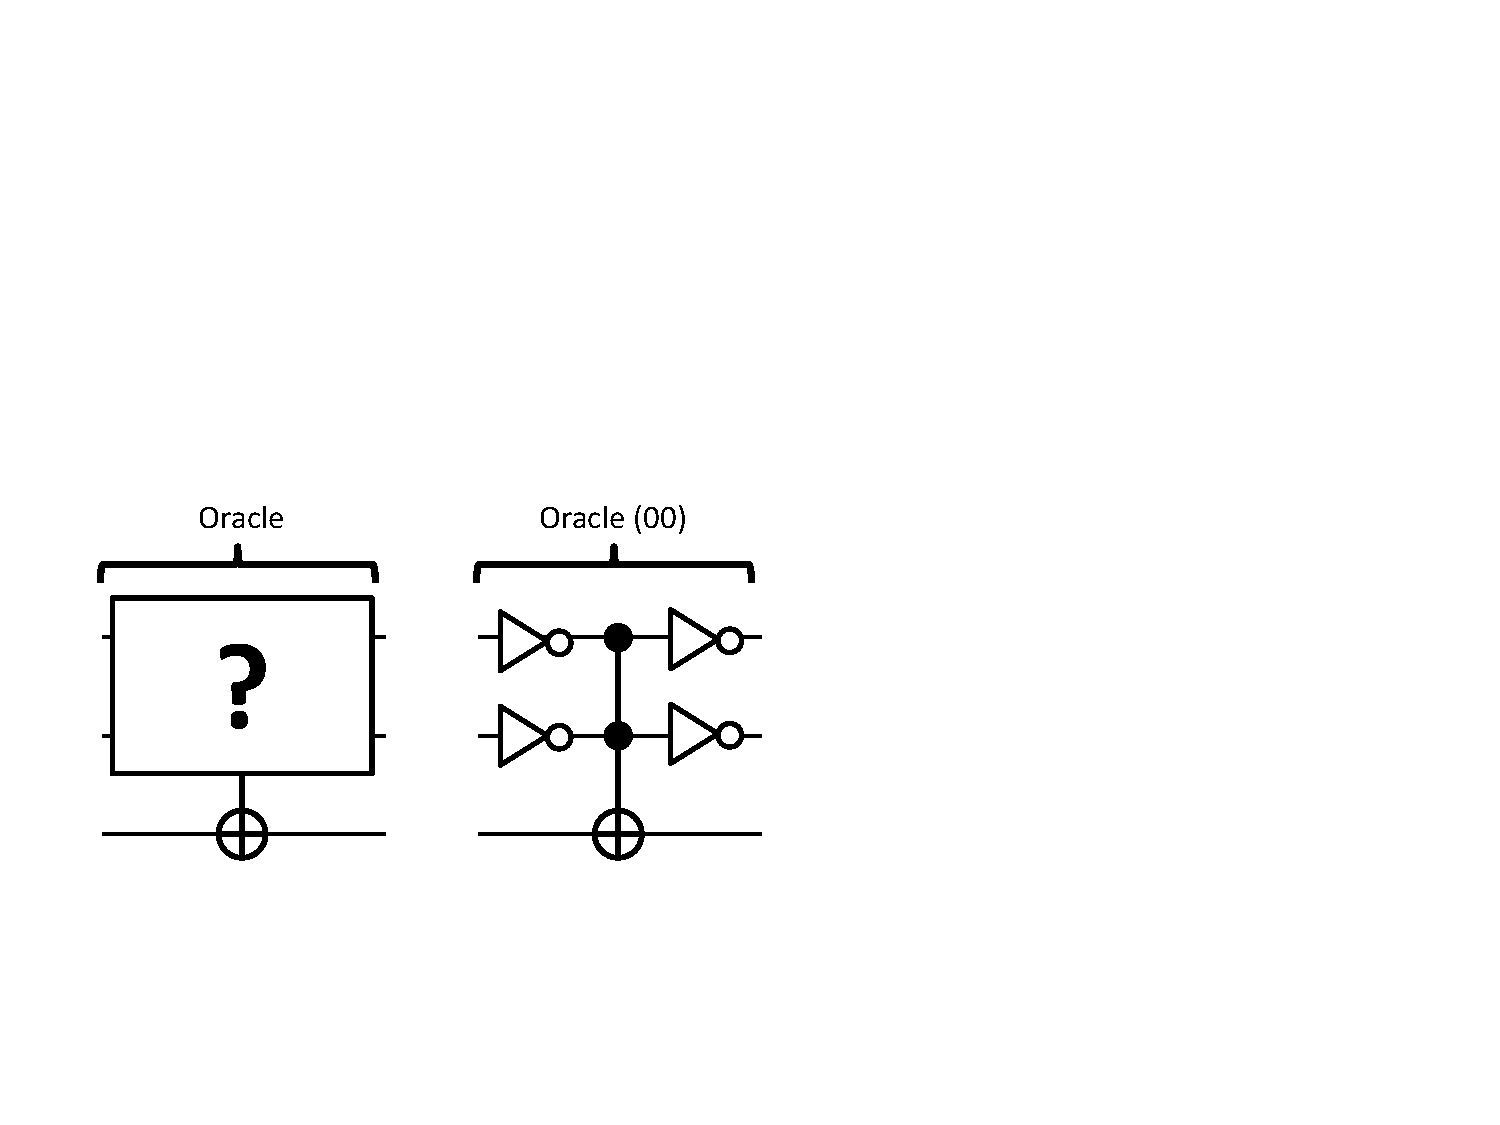
\includegraphics[width=0.5\textwidth]{./material/papers/grover/different_oracle_implementations}
	\caption[]{a) Ancilla-based implementation of the Oracle function $\Or$. The state of the third bit get flipped if the search function $\Or(i)=1$ for the given input state $i$. b) An example of an ancilla-based search function that returns a true value for the input state $00$.}
	\label{fig:GroverOracleImplementations}
\end{SCfigure}

Exemplary implementations of ancilla-based search functions $\Or$ implemented using reversible (quantum) gates are shown in fig. \ref{fig:GroverOracleImplementations} for the two-qubit case. There, a two-qubit Tofolli gate in combination with several single-qubit NOT gates (that can be easily implemented as single-qubit $X_{\pi}$ rotations) is used to flip the state of an ancilla-qubit conditionally on the input state of the gate. Using this approach, any arbitrary classical search function $\Or$ that can be implemented with a set of universal reversible logic gates (e.g. the Toffoli gate and the NOT gate) can be directly mapped to a corresponding quantum operator that works on quantum-mechanical input states and implements the classical search function.

\begin{figure}[ht!]
	\centering
		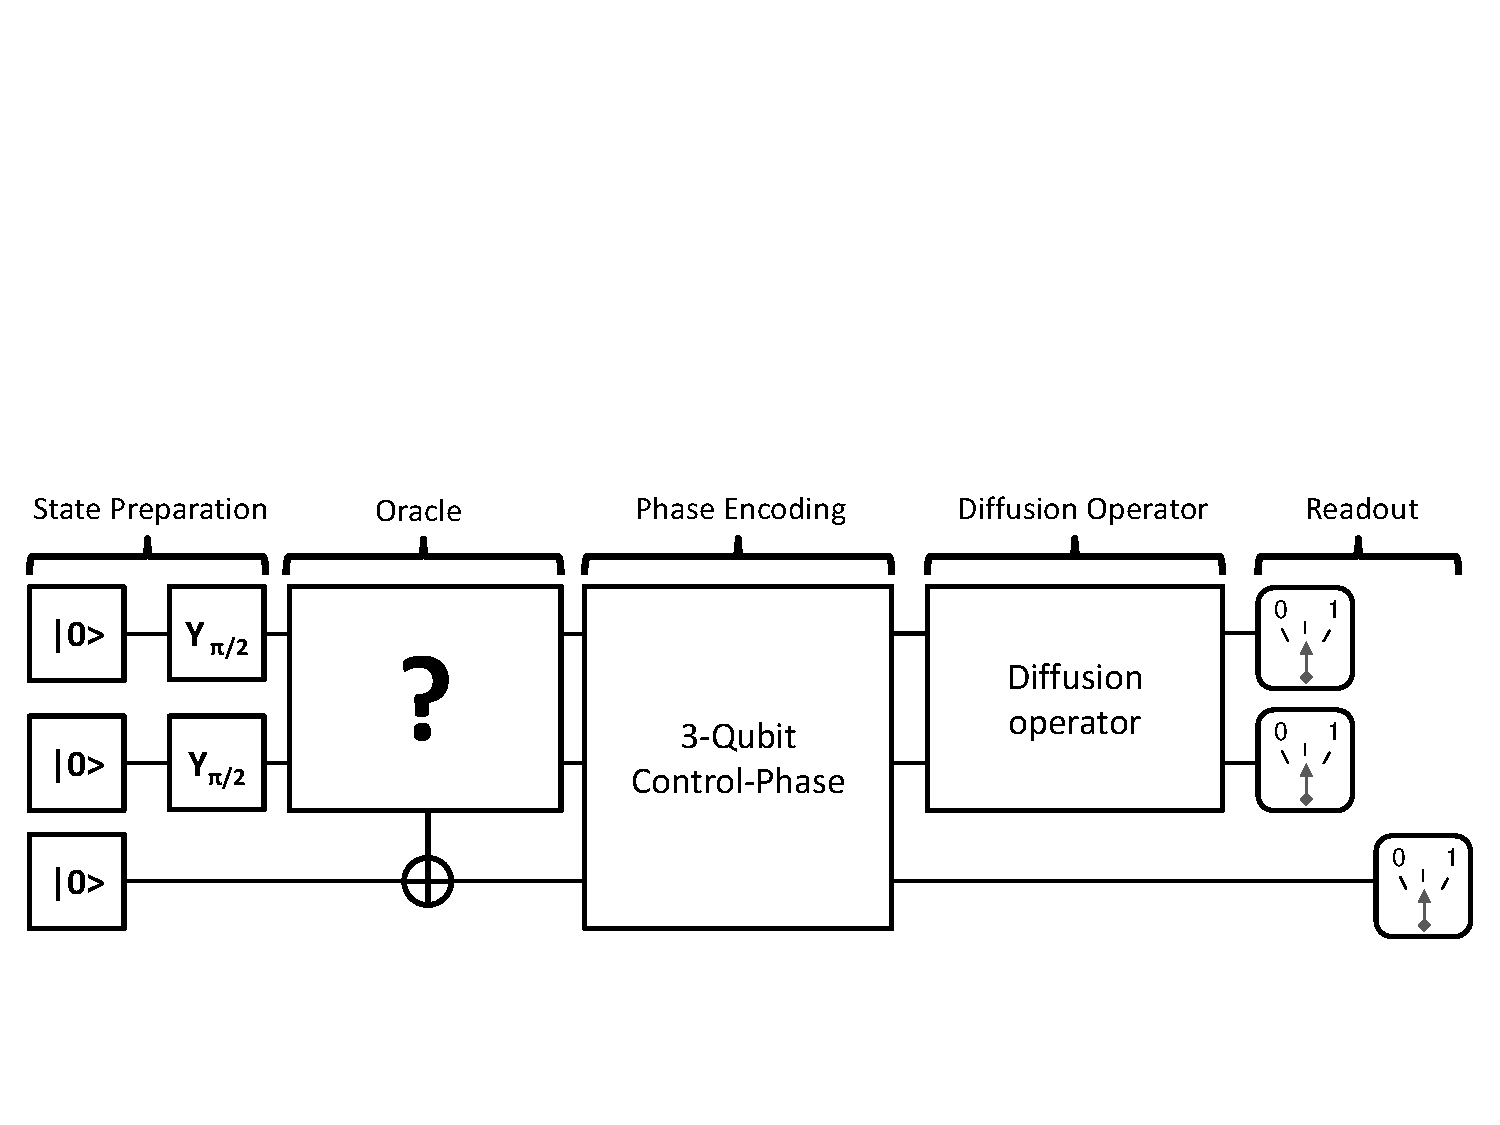
\includegraphics[width=1\textwidth]{./material/papers/grover/quantum_algorithm_full}
	\caption[Full version of an ancilla-based implementation of the two-qubit Grover search algorithm]{A full version of an ancilla-based implementation of the two-qubit Grover search algorithm. The algorithm works on a two-qubit input state and flips the state of a control qubit for one of the four possible input states in accordance to an unknown Oracle function. It then applies a 3-qubit control-phase operation of that maps $\ket{xx1}\to -\ket{xx1}$, $\ket{xx0}\to\ket{xx0}$ to encode the state of the control qubit directly in the two input qubits and then uses a diffusion operator to determine the state which has been marked by the Oracle function.}
	\label{fig:GroverAlgorithmFullSchematic}
\end{figure}

\smallskip

Now, to use the Grover algorithm with such an ancilla-based quantum Oracle, it is neccessary to re-encode the result of the Oracle in the qubit input state. Fig. \ref{fig:GroverAlgorithmFullSchematic} shows a version of the two-qubit Grover algorithm that achieves exactly this by using a three-qubit control-not (CNOT) gate $C$ of the form
%
\begin{equation}
C = \mathrm{I}^{n\otimes n}-2\sum\limits_{ij} \ket{ij1}\bra{ij1}
\end{equation}
%
to phase-encoded the state of the anciall qubit in the state of the input qubit register. After the re-encoding of the result, the ancilla qubit is not needed during the remainder of the algorithm and must not be read out before the algorithm terminates.

\section{Comparision to a Classical Algorithm}

\begin{figure}[ht!]
	\centering
		\includegraphics[width=1.0\textwidth]{"./material/papers/grover/classical_reversible_algorithm"}
	\caption{Classical reversible implementation of a search algorithm on a two-bit input register. The Oracle function can be implemented by two single-bit NOT operations and a Toffoli gate. R designates the generation of a random binary value at the beginning of the algorithm. If the Oracle does not yield the correct answer, the test state is incremented. The average success probability of the algorithm is 50 \%.}
	\label{fig:GroverClassicalReversibleAlgorithm}
\end{figure}

In order to quantify the quantum speed-up achieved by a quantum algorithm it is necessary to map the problem it solves to an equivalent problem that can be solved by a classical algorithm. For the Grover algorithm, this is the search problem that we discussed in the first section of this chapter. Now, with the ancilla-based version of the Grover algorithm introduced in the last section it is possible to directly formulate a classical algorithm that solves the same problem and compare the efficiency of the two. We can use reversible logic gates such as the Toffoli gate and the single-(qu)bit NOT gate to implement the classical algorithm, thereby achieving a maxmimum comparability with the quantum version. Since the two-qubit Grover algorithm evaluates the search function $\Or$ only once it is interesting to ask what would be the performance of an equivalent classical algorithm which calls $\Or$ once and returns an estimate of the state solving the search problem. Such an algorithm is shown in fig. \ref{fig:GroverClassicalReversibleAlgorithm}. It achieves a success probability of 50 \% by evaluating the function $\Or$ for a randomly generated two-bit input value $r$ and returning $r$ if it found $\Or(r)=1$ or $r+1(\mathrm{mod}\;4)$ otherwise. The 50 \% success rate of this algorithm provides a benchmark against which we will measure the speed-up of our implementation of the Grover algorithm.


\section{Experimental Implementation}

\begin{figure}[ht!]
	\centering
		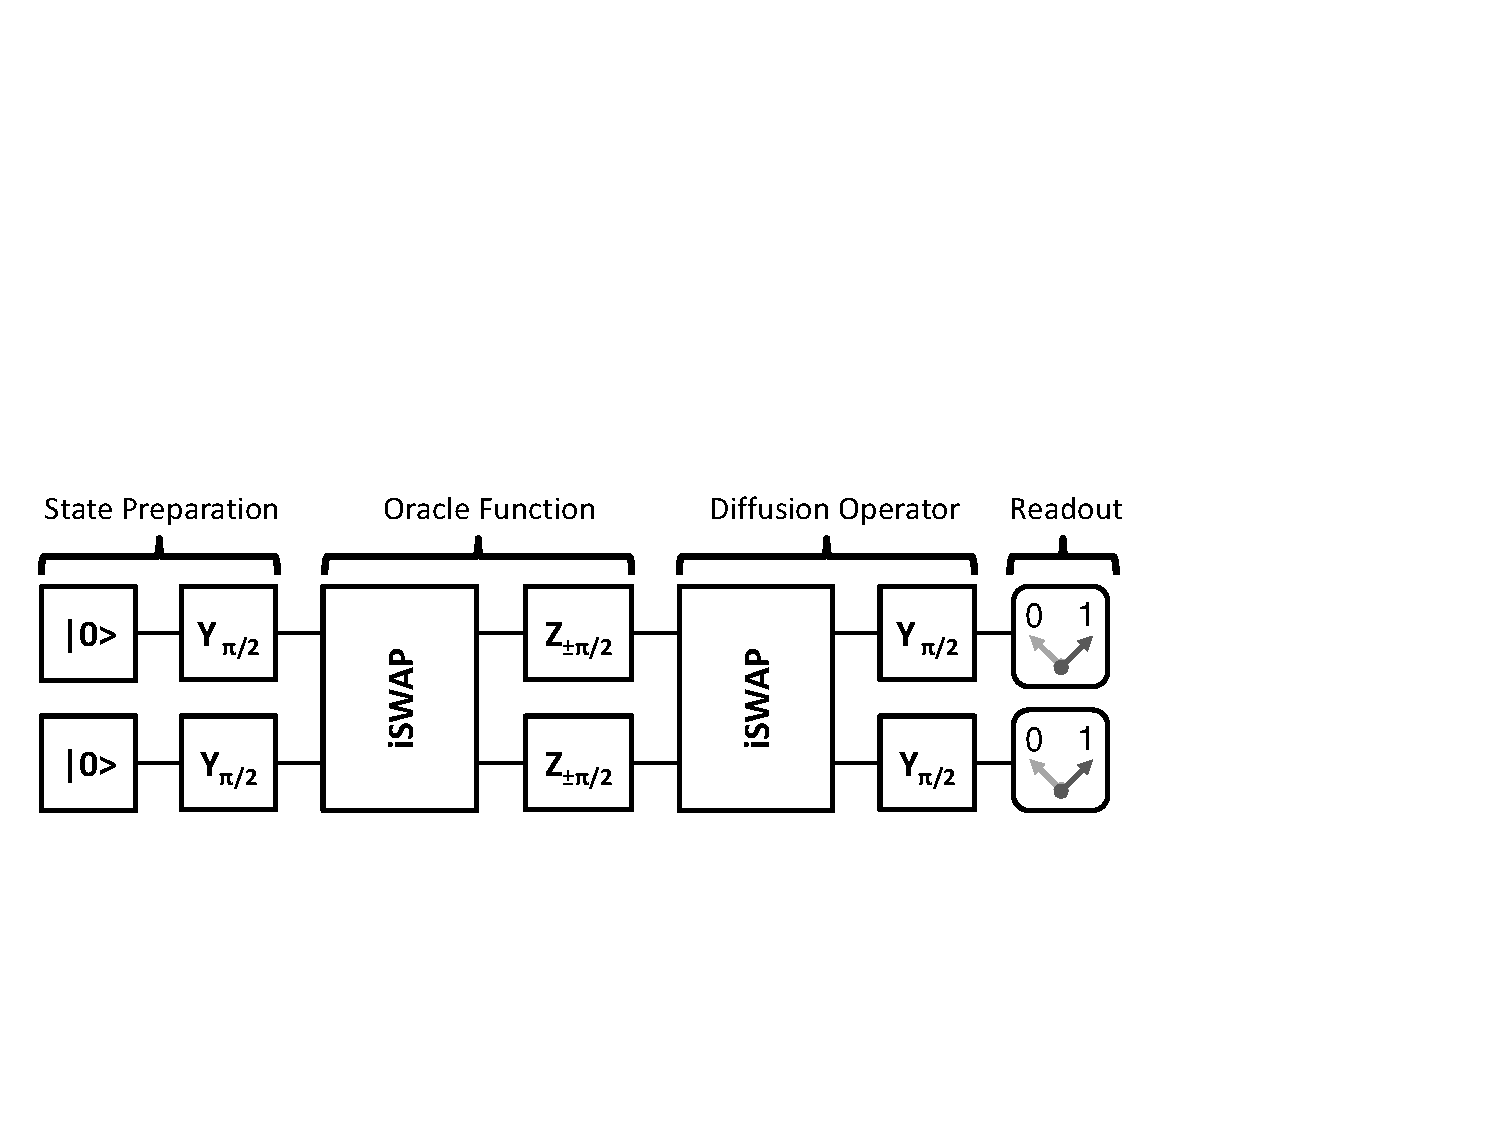
\includegraphics[width=0.8\textwidth]{./material/papers/grover/grover_algorithm}
	\caption[Schematic of our implementation of the Grover search algorithm]{Schematic of our implementation of the Grover search algorithm. The algorithm consists in generating a fully superposed input state, applying the Oracle function to it and analyzing the resulting state by applying the Diffusion transform to it and reading out the value of the qubit register afterwards.}
	\label{fig:GroverAlgorithmSchematic}
\end{figure}

In this work we implement a compiled version of the two-qubit Grover algorithm. The gate sequence of the algorithm is shown in fig. \ref{fig:GroverAlgorithmSchematic} and consists in two $i\mathrm{SWAP}$ gates and six single-qubit gates applied to an initial state $\ket{00}$. The first $i\mathrm{SWAP}$ gate together with the two single-qubit $Z_{\pm \pi}$ rotations implements the Oracle function $f(x)$ as given in eq. (\ref{eq:GroverOracleFunction}), where the signs of the rotation operations determines the state which is marked and can be either $\ket{00}$ (corresponding to a $Z^1_{-\pi/2}\cdot Z^2_{-\pi/2}$ rotation), $\ket{01}$ ($Z^1_{-\pi/2}\cdot Z^2_{\pi/2}$), $\ket{10}$ ($Z^1_{\pi/2}\cdot Z^2_{-\pi/2}$) or $\ket{11}$ ($Z^1_{\pi/2}\cdot Z^2_{\pi/2}$). The second $i\mathrm{SWAP}$ operation together with the following $X^1_{\pi/2}\cdot X^2_{\pi/2}$ operation implements the difussion operator as given by eq (\ref{eq:GroverDiffusionOperator}). The final step of the algorithm consists in reading out the two-qubit register.

\subsection{Pulse Sequence}

To implement the gate sequence described above we need to realize a sequence of microwave and flux pulses which realize the individual quantum gates of the sequence. To eliminate possible gate errors, we perform a series of calibration measurements before to tune-up the individual single- and two-qubit gates needed for the algorithm. In addition, we run individual parts of the algorithm successively and perform quantum state tomography to characterize the state of the quantum register after each step of the algorithm and correct the gate operations applied to the qubit in order to maximize the fidelity of the measured states in respect to the ideal ones. Fig. \ref{fig:GroverPulseSequence} shows an experimental pulse sequence for the Grover algorithm with an Oracle operator marking the state $\ket{00}$. Shown are the frequencies of the two qubits during the runtime of the algorithm and the microwave drive and readout pulses applied to them.

\begin{figure}[htb!]
	\centering
		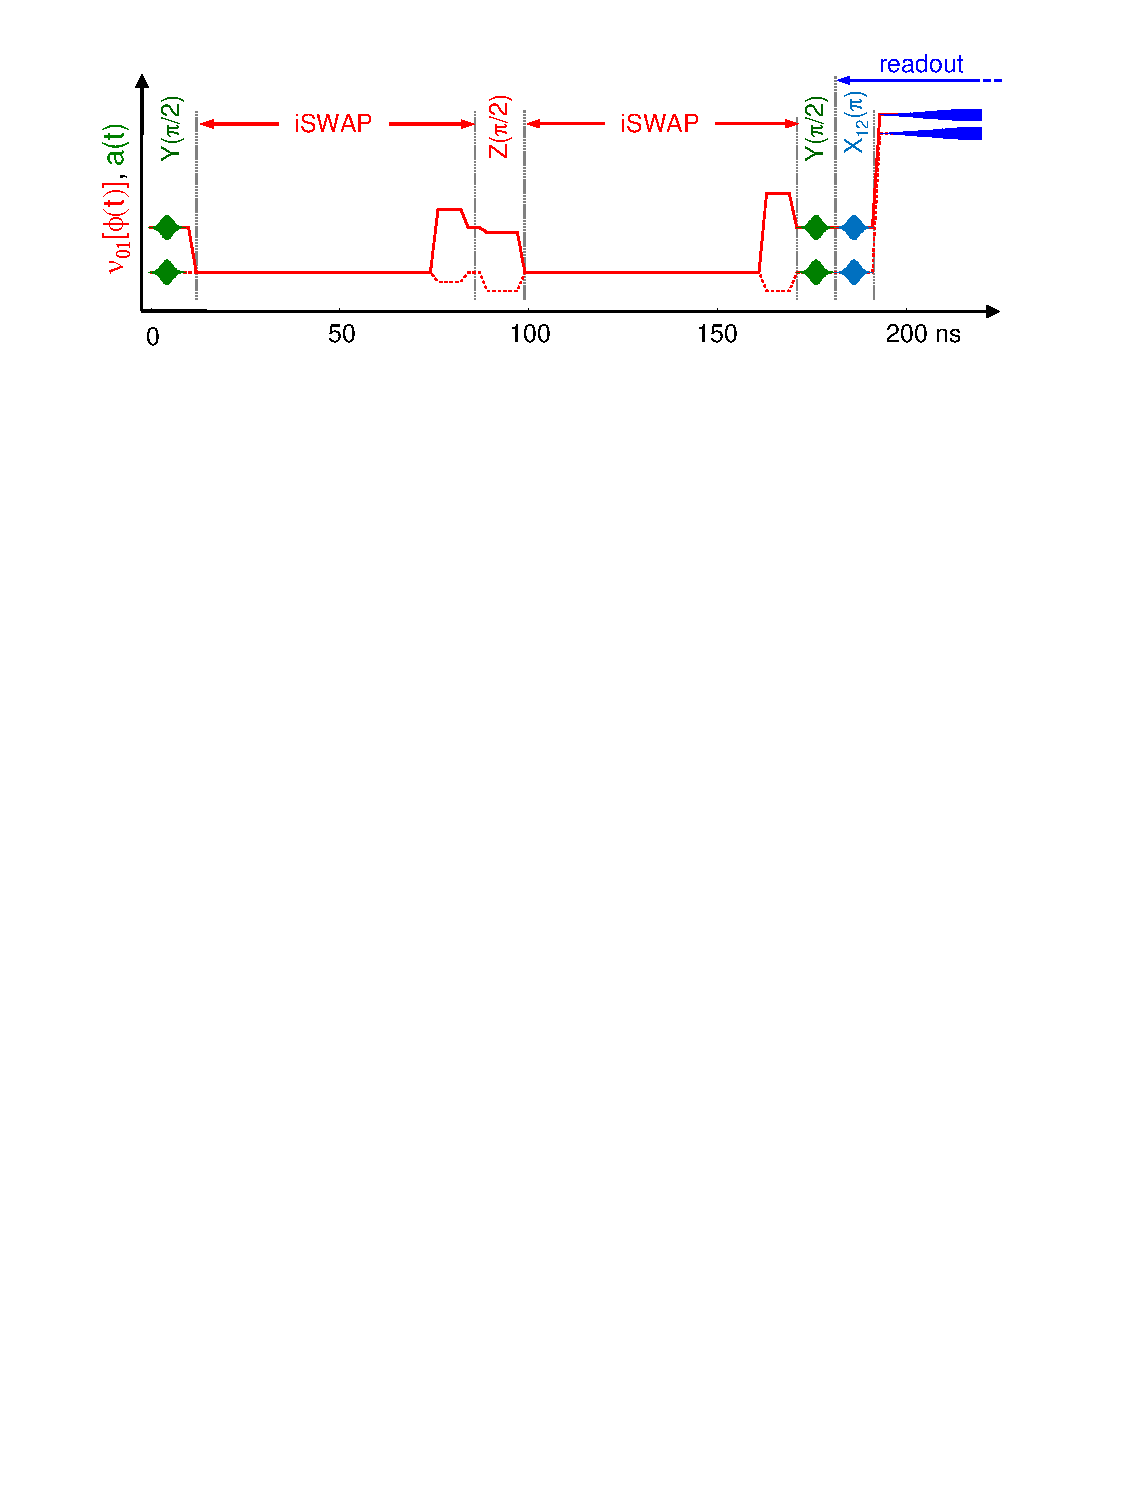
\includegraphics[width=1.\textwidth]{./material/papers/grover/figures/grover_algorithm_pulse_sequence}
	\caption[Pulse sequence used for implementing Grovers search algorithm]{The pulse sequence used in realizing Grover's quantum search algorithm. First, a $Y_{\pi/2}$ pulse is applied to each qubit to produce the fully superposed state $1/2(\ket{00}+\ket{01}+\ket{10}+\ket{11})$. Then, an $i\mathrm{SWAP}$ gate is applied, followed by a $Z_{\pm \pi /2}$ gate on each qubit, which corrsponds to the application of the oracle function. The resulting state is then analyzed using another $i\mathrm{SWAP}$ gate and two $X_{\pi/2}$ gates to extract the state which has been marked by the oracle function. Optionally, a $Y^{12}_{\pi}$ pulse is used on each qubit to increase the readout fidelity.}
	\label{fig:GroverPulseSequence}
\end{figure}

\section{Results}

Here we discuss the results obtained when running the Grover search algorithm with our two-qubit processor. In the first section we will analyze the quantum state of the qubit register during the algorithm by performing quantum state tomography. In the second section we will present and discuss the single-run results obtained in our experiment.

\subsection{State Tomography of the Algorithm}

Fig. \ref{fig:GroverAlgorithmExperimentalResults} shows the results when running the Grover search algorithm for the four possible Oracle functions. Shown are quantum state tomographies after each step of the algorithm and the single-run results obtained when measuring the qubit register after the final step of the algorithm. In subfigures  (a)-(d) The black outlined circles in the density matrices represent the ideal theoretical states, whereas the colored, solid circles represent the experimentially measured states. The trace fidelities of all states with the ideal ones are noted above each density matrix. As can be seen, the fidelity diminshes as a function of the runtime of the algorithm due to dephasing and relaxation of the qubit register. The experimental single-shot probabilities in subfigure (e) are shown along with the expected probabilities, which are calculated based on the readout matrix of our two-qubit system and the state tomographies after the final state of the algorithm. 

\begin{figure}[ht!]
	\centering
		\includegraphics[width=1.\textwidth]{"./data/ct5/2011_04_21 - grover and tomo/good_data/grover algorithm - single run results - density matrices only"}
	\caption[Quantum state tomographies at different steps during the Grover search algorithm and single-run outcome probabilities]{Quantum state tomographies at different steps of the Grover search algorithm. The density matrices show the experimentally measured states in color and the theoretical states in black. For each state, the trace fidelity $F_{tr}(\rho_A,\rho_B) = \mathrm{Tr}\{\rho_A\cdot\rho_B\}$ is shown above the density matrix.}
	\label{fig:GroverAlgorithmExperimentalResults}
\end{figure}

\subsection{Single Run Results}

\begin{figure}[htb!]
	\centering
		\includegraphics[width=1.\textwidth]{"./data/ct5/2011_04_21 - grover and tomo/good_data/grover algorithm - single run probabilities"}
		\caption[Single-run success probabilities of the Grover search algorithm]{The single-run success probabilities of our implementation of the Grover search algorithm. Shown are the averaged probabilities for the four possible Oracle functions. The red bars correspond to measured values, the blue ones to expected probabilities calculated using the reconstructed density matrices after the final step of the algorithm and the measured two-qubit readout matrix. The dashed line indicates the average success probability of a classical query-and-guess algorithm for comparision.}
	\label{fig:GroverSingleShotResults}
\end{figure}

The experimental state tomographies discussed in the last section show that we are able to implement the Grover search algorithm with adequate fidelity using our two-qubit processor. However, the analysis of the two-qubit register by quantum state tomography at the end of the algorithm does not prove that we can achieve real quantum speed-up with our processor. For this, it is necessary to directly read out the state of the qubit register at the end of the algorithm {\it without} performing any kind of error correction afterwards. By looking at this ``raw'' outcome data and averaging it over many identical runs of the processor we can then quantify the success rate and the fidelity of the algorithm we implemented. The results of such measurements that we performed for the four possible Oracle functions is shown in fig. \ref{fig:GroverSingleShotResults}. Besides the single-run probabilities for all four Oracle functions, the diagram also shows for comparision the expected outcome probabilities that are calculated based on the quantum state tomographies discussed above and the readout matrix of the two-qubit system. As can be seen, the agreement between the measured and calculated probabilities is quite good. The dashed line in the diagrams corresponds to the success probability of a classical ``query-and-guess'' algorithm as described above, which is bound to 50 \% and provides the benchmark against which we measure the quantum speed-up in this system. As can be seen, our implementation of the Grover search algorithm outperforms a classical search algorithm for all four Oracle functions, if only by a small margin.

\section{Algorithm Fidelity}

We can define the average fidelity of the algorithm in a single run, which corresponds to the averaged success probabilities measured for all four Oracle functions and averaged over a large sample set. Table \ref{tab:Probabilities-for-obtaining} shows these single-run probabilities along with the so-called {\it user fidelities}, which are given as
%
\begin{equation}
f_{ab} = p(\ket{ab}|ab) = \frac{p(ab |\ket{ab})}{\sum\limits_{uv}p(uv|\ket{uv})} 
\end{equation}
%
and correspond to the probability of having obtained the correct answer given a certain outcome, averaged over all four possible Oracle functions. For all four, both the single-run and user fidelities are $> 50 \%$, hence demonstrating quantum speed-up in comparision with a classical query-and-guess algorithm as discussed above.

\begin{table}[H]
\begin{centering}
\begin{tabular}{|c|c|c|c|c|c|c|}
\hline 
$ab$/$|uv\rangle$ & $\left|00\right\rangle $ & $\left|01\right\rangle $ & $\left|10\right\rangle $ & $\left|11\right\rangle $ & $\sum$ & $f_{ab}$\tabularnewline
\hline
\hline 
00 & \textcolor{red}{0.666} & 0.192 & 0.188 & 0.122 & 1.168 & 57.0 \%\tabularnewline
\hline 
01 & 0.127 & \textcolor{red}{0.554} & 0.071 & 0.122 & 0.874 & 63.4 \%\tabularnewline
\hline 
10 & 0.128 & 0.106 & \textcolor{red}{0.615} & 0.239 & 1.088 & 56.5 \%\tabularnewline
\hline 
11 & 0.079 & 0.148 & 0.126 & \textcolor{red}{0.517} & 0.870 & 59.4 \%\tabularnewline
\hline
\end{tabular}
\par\end{centering}

\caption{\label{tab:Probabilities-for-obtaining}Conditional probabilities
$p_{ab/|uv\rangle}$ and statistical fidelities $f_{ab}$ for all
possible outcomes $ab$, measured for our version of Grover's algorithm.}

\end{table}

\section{Error Analysis}

There are three kind of errors arising in our implementation of the Grover search algorithm that we will analyze in the following section. These errors are:

\begin{enumerate}
	\item Deterministic, unitary gate errors
	\item Stochastic errors introduced due to qubit decoherence during the runtime of the algorithm
	\item Readout errors due to qubit relaxation during the readout of the qubit state, insufficient coupling between the qubit and the readout or retrapping of the readout state during measurement
\end{enumerate}

We will analyze the contributions of all these three error sources for the implementation of the algorithm below.
\subsection{Gate Errors \& Decoherence}

Gate errors are unitary errors that arise due to misshaped or mistuned gate pulses. Usually the effect of these errors is combined with stochastic, non-unitary errors arising due to qubit decoherence during the runtime of the algorithm and therefore has to be analyzed together with the latter. Hence, in order to quantify these errors it is necessary to generate an error model of our algorithm that takes into account both unitary as well as non-unitary errors and whose parameters we obtain by fitting the model to our experimental results. Repeating this procedures for the experimental runs implementing the four different Oracle functions we obtain a full quantitative error model for all of them.

\subsubsection{Modeling Decoherence}

We could again model decoherence processes in our algorithm by formulating an effective master equation of the two-qubit system that includes relaxation and dephasing processes as we did when anylyzing the universal quantum gate that we implemented. For our implementation of the Grover algorithm, however, we chose to rather use a set of discrete decoherence operators that model amplitude (i.e. $T_1$) and phase daming (i.e. $T_\phi$) processes and which we can directly integrate in a more simple, operator-based model of the algorithm. We can then model the decoherence in our algorithm by applying these operators to the calculated quantum states after each individual step of the algorithm. Like this we can generate an error model incorporating the most relevant experimental decoherence processes without the need to numerically integrate an effective master equation, thereby greatly speeding up the process of fitting our experimental data to the formulated error model. In the following paragraphs we introduce the reader to the operators we use to model relaxation and dephasing processes in our error model.

\smallskip

To model qubit relaxation, we can use a pair of single-qubit operators describing amplitude-daming of the qubit state, which given as \citep{michael_a._nielsen_quantum_2000}
%
\begin{align}
 E_1^{T_1} & = \left(\begin{array}{cc} 1 & 0 \\ 0 & \sqrt{1-\gamma_{T_1}} \end{array}\right)   &  E_2^{T_1}  & = \left( \begin{array}{cc} 0 & \sqrt{\gamma_{T_1}} \\ 0 & 0 \end{array} \right) \label{eq:grover_energy_relaxation}
\end{align}
%
On the other hand, phase-daming operators describing qubit dephasing can be written analogously as
%
\begin{align}
 E_1^{T_{\phi 1}} & = \left(\begin{array}{cc} 1 & 0 \\ 0 & \sqrt{1-\gamma_\phi} \end{array}\right)   &  E_2^{T_{\phi 1}}  & = \left( \begin{array}{cc} 0 & 0 \\ 0 & \sqrt{\gamma_\phi}  \end{array} \right) \label{eq:grover_phase_decoherence}
\end{align}
%
Both operators are applied to a quantum state $\rho$ according to
%
\begin{equation}
\rho \to E_1 \rho E_1^\dagger+E_2 \rho E_2^\dagger
\end{equation}
%
and yield a trace-preserving, non-unitary evolution of the quantum state of $\rho$. The decoherence fraction $\gamma$ that is used in the operators can be calculated from the corresponding relaxation and dephasing rates as $\gamma_{T_{1,2}}(t) = 1-\exp{\left(-t \Gamma_{1,2}^{T_1}\right)}$ and $\gamma_{\phi_{1,2}} = 1-\exp{\left(-t \Gamma_{1,2}^{T_\phi}/2\right)}$, where $t$ is the time during which the state is exposed to the given decoherence process.

\smallskip

\begin{figure}[ht!]
	\centering
		\includegraphics[width=0.85\textwidth]{"./material/papers/grover/grover_error_model"}
	\caption[Error model used for analyzing gate and decoherence errors for the Grover search algorithm]{The error model we use to analyze the different gate and decoherence errors present when running the Grover search algorithm. The dotted lines indicate the points at which the quantum state has been measured by state tomography.}
	\label{fig:GroverErrorModel}
\end{figure}


Using these two operators combined with a set of unitary operators describing the quantum operations performed during the algorithm we formulate a full error model that we use to model our experimental data, as shown in fig. \ref{fig:GroverErrorModel}. This model takes into account the following error sources:

\begin{itemize}
 \item {\bf Energy relaxation and phase decoherence}: Energy relaxation and dephasing of the qubit is modeled using the processes given in eqs. (\ref{eq:grover_energy_relaxation}) and (\ref{eq:grover_phase_decoherence}), applying these operators with an adapted $\gamma$ after each unitary operation performed during the algorithm.
 \item {\bf Single-qubit gate errors}: We model rotation angle and rotation phase errors of our single-qubit $X_\alpha$ and $Y_\alpha$ gates by replacing them with operators of the form $X_\alpha\to \phi_{\alpha'} = \cos{\phi}X_{\alpha'}+\sin{\phi}Y_{\alpha'}$ and $Y_\alpha \to \varphi_{\alpha'} = \sin{\varphi}X_{\alpha'}+\cos{\varphi}Y_{\alpha'}$. For $Z$-type single-qubit operators we model only rotation angle errors by replacing $Z_\alpha \to Z_{\alpha'}$ 
 \item {\bf Two-qubit gate errors:} We model both detuning and gate-length errors of our $i\mathrm{SWAP}$ 2-qubit gates.
\end{itemize}

For the two-qubit gates, we model the errors present in the $i\mathrm{SWAP}$ operation by using the model
%
\begin{equation}
i\mathrm{SWAP}(t,\Delta) = \left(
			\begin{array}{cccc}
				1 & 0 & 0 & 0 \\
				0 & \cos{t g_{e}}-i\frac{\Delta}{g_{e}}\sin{t g_{e}} & i \frac{g}{g_e}\sin{t g_{e}} & 0 \\
				0 & i\frac{g}{g_e}\sin{t g_{e}} & \cos{t g_{e}}+i\frac{\Delta}{g_{e}}\sin{t g_{e}} & 0 \\
				0 & 0 & 0 & 1 \\
			\end{array}
	\right) \label{eq:swap_with_detuning}
\end{equation}
%
\begin{figure}
	\centering
		\rotatebox{90}{\includegraphics[width=1.2\textwidth]{"./data/ct5/2011_04_21 - grover and tomo/good_data/grover - simulated density matrices with errors"}}
	\caption[Comparision of the general error model to our experimental data]{Comparision of the fitted error model as given by eq. (\ref{eq:grover_error_model}) to our experimental data. Experimental data is shown in color, the fitted density matrices as black outlines. As before, we show the state fidelity according to eq. (\ref{eq:state_fideltiy}) between experimental and fitted states.}
	\label{fig:grover_error_model}
\end{figure}

where $g_e = \sqrt{g^2+\Delta^2}$ is the effective swap frequency at a qubit frequency detuning $f_{01}^1-f_{01}^2 = 2\Delta$. Often it is pratical to replace $t$ and $\Delta$ with $\beta = t g_{e}$ and $\delta = \Delta / g$. Using this notation of the iSWAP gate and the definition of the single-qubit gates as discussed before, the full algorithm with gate errors can be written as (for right-multiplication)
%
\begin{equation}
\mathrm{Grover} = \phi_{\gamma_1}^1\otimes \phi_{\gamma_2}^2\cdot i\mathrm{SWAP}(\epsilon_2,\delta_2)\cdot Z_{\beta_1}\otimes Z_{\beta_2}\cdot i\mathrm{SWAP}(\epsilon_1,\delta_1)\cdot\varphi_{\alpha_1}^1\otimes \varphi_{\alpha_2}^2 \label{eq:grover_error_model}
\end{equation}
%
In addition, we add a dephasing and relaxation error after each step of the algorithm to model the decoherence during the runtime of the algorithm. Numerical optimization is then used to produce a fit of all the gate errors, which is shown in tab. \ref{tab:grover_error_parameters}. Here, the qubit relaxation and dephasing times were measured independently and are not part of the fit.

\begin{table}[ht!]
\centering
\footnotesize{
\begin{tabular}{r|rrrrrrrrrrrrrr}
state & $\delta_1$ & $\delta_2$ & $\alpha_1$ & $\alpha_2$ & $\varphi_1$ & $\varphi_2$ & $\epsilon_1$ & $\beta_1$ & $\beta_2$ & $\epsilon_2$ & $\gamma_1$ & $\gamma_2$ & $\phi_1$ & $\phi_2$ \\ \hline
$\ket{00}$ & 0.06 & -0.06 & -2.5 & 2.7 & 6.1 & 3.1 & -7.3 & -3.3 & -4.1 & 7.5 & 29 & 9.3 & 0.66 & -1.7
 \\
$\ket{01}$ & 0.04 & -0.3 & -0.1 & 0.1 & 7.9 & 3.6 & -11 & -5.9 & 2.2 & -6.9 & 28 & -19 &  9 &  2
 \\
$\ket{10}$ & 0.09 & -0.2 & -3.1 & 1.7 &  1 & -2.5 & -6.5 & -15 & -22 & -7.5 & -15 & 32 & 3.6 & 5.2
\\
$\ket{11}$ & 0.16 & 0.13 & -6 & 3.9 & 2.2 & 0.9 & -9.5 & -20 & -15 & 17 & -12 & -32 & -7 & -8.9
\end{tabular}
}
\caption[Fitted gate error parameters of the Grover algorithm]{Fitted error parameters for the measured density matrices, modeled according to the error model given in eq. (\ref{eq:grover_error_model}). Alle angles are given in $\deg$.}
\label{tab:grover_error_parameters}
\end{table}

The resulting fitted error models obtained for our experimental data are shown in tab. \ref{tab:grover_error_parameters}. As can bee seen, the phase and gate-time errors for the first gates are comparatively small and grow bigger during the following steps of the algorithm. Curiously, the phase errors are bigger for the states $\ket{10}$ and $\ket{11}$, as are the gate-length errors for the two $i\mathrm{SWAP}$ gates used in the algorithm. This fact might be explained by a drift of the operating point of our microwave setup during the time it took to take the data for the four possible Oracle operators, during which the parameters of individual qubit gates were not recalibrated.

\smallskip

Fig. \ref{fig:grover_error_model} shows again the measured density matrices for our realization of the Grover search algorithm, this time overlaid with the numerically optimized error model according to eq. (\ref{eq:grover_error_model}). As can be seen, our error model is able to capture most of the observed experimental errors and can reproduce to very good accuracy the observed density matrices. The state fidelities according to eq. \ref{eq:state_fidelity} between the measured density matrices and those of the fitted error model are shown above each density matrix.

\subsubsection{Fidelity of the Oracle and diffusion operators}

It is interesting to analyze the individual experimental fidelities of the Oracle and diffusion operators that make up the Grover algorithm achieved in our experiment. For this, we compare the action of the ideal operators $D'$ and $R'$ with that of the experimentally implemented versions $D'_{e}$ and $R'_{e}$, taking the measured quantum states before applying each of the operators as input. We take then as the fidelity of each operator the average state fidelity of the measured output states as compared to the calculated ones, i.e.
%
\begin{eqnarray}
F(D'_{e}) & = & F(D'\rho_{in}D^{'\dagger},D'_e \rho_{in} D_{e}^{'\dagger}) \label{eq:grover_diffusion_fidelity} \\
F(R'_{e}) & = & F(R'\rho_{in}R^{'\dagger},R'_e \rho_{in} R_{e}^{'\dagger}) \label{eq:grover_oracle_fidelity}
\end{eqnarray}
%
where we also make use of the state fidelity according to eq. \ref{eq:state_fidelity}. By this method, we obtain the following experimental fidelities for the two gate operations:

\begin{table}[ht!]
\centering
\begin{tabular}{r|rrrr|l}
Operator / State & $\ket{00}$ & $\ket{01}$ & $\ket{10}$ & $\ket{11}$ & Average \\ \hline 
$D'$ & 92.3 & 93.4 & 94.3 & 91.7 & 92.9 \\
$R'$ & 94.5 & 93.6 & 88.5 & 87.7 & 91.1
\end{tabular}
\caption[Measured fidelities of the quantum Oracle and diffusion operators used in the Grover search algorithm]{Measured fidelities of the quantum Oracle and diffusion operators used in the Grover search algorithm according to eqs. (\ref{eq:grover_diffusion_fidelity}) and (\ref{eq:grover_oracle_fidelity}). All fidelities are given in percent.}
\end{table}

As can be seen, on average we are able to implement both the diffusion operator and the quantum Oracle with a fidelity $>90\%$.
\subsection{Readout Errors}

\begin{figure}[ht!]
	\centering
\includegraphics[width=0.19\textwidth]{"./data/ct5/2011_04_21 - grover and tomo/good_data/single qubit readouts"}
\includegraphics[width=0.79\textwidth]{"./data/ct5/2011_04_21 - grover and tomo/good_data/readout and crosstalk - 2 plots"}
	\caption[Measured single- and two-qubit readout matrices and crosstalk matrix for the Grover search algorithm experiment]{a.)The measured single-qubit readout matrices, showing the readout outcome probabilities as a function of the prepared state for both qubits. b.)The measured two-qubit readout matrix, showing again the detector outcome probabilities versus the prepared qubit states. c.) The crosstalk matrix, corresponding to the product of the inverse two-qubit readout matrix and the Kronecker product of the single-qubit readout matrices. Note that the $\ket{1}\to\ket{2}$ shelving method is used for reading out the qubit state, which increases readout fidelity but also inter-qubit readout crosstalk.}
	\label{fig:GroverReadoutMatrix}
\end{figure}

Another source of errors affecting the single-run fidelities of the algorith arises due to the imperfection of our qubit readout. Here, mostly qubit relaxation during the readout process reduces the visibility of individual qubit states and introduces errors when reading out the qubit register in the final step of the algorithm. We can easily quantify those readout errors by using the readout matrix that was introduced in the last chapter. When running the Grover algorithm we use the $\ket{1}\to\ket{2}$ shelving method described in the last chapter to increase the readout contrast and thereby the algorithm fidelity. This technique reduces single-qubit readout errors but increases inter-qubit readout crosstalk. To quantify all single-qubit and inter-qubit readout errors, we first model the readout matrix $R$ of the two-qubit system as a product $R=R_{v}\cdot R_{ct}$, where $R_{v}$ is the so-called {\it visibility matrix} and $R_{ct}$ a matrix describing the readout crosstalk. The visibility matrix can be written as the Kronecker product $R_{v} = R_{v}^1 \otimes R_{v}^2$ of the two single-qubit readout matrices, which have the form
%
\begin{equation}
R_{v}^{1,2} = \left(
			\begin{array}{cc}
				p_{00}^{1,2} & 1-p_{11}^{1,2} \\
				1-p_{00}^{1,2} & p_{11}^{1,2}
			\end{array}
		\right)
\end{equation}
%
Here, $p_{00}^{1,2}$ ($p_{11}^{1,2}$) corresponds to the probability to measure the value $0$ ($1$) at the readout after having prepared the qubit in state $\ket{0}$ ($\ket{1}$). Usually, the full two-qubit readout matrix $R$ and the single-qubit readout matrices $R_{v}^{1,2}$ are measured experimentially which allows us then to calculate the crosstalk matrix as $R_{ct} = R_{v}^{-1}\cdot R$. The three matrices measured in our experiment are shown in fig. \ref{fig:GroverReadoutMatrix}. As can be seen, the single-qubit readout fidelities range between 87 - 96 \% and the combined two-qubit readout fidelities between 75 - 85 \%. Depending on the qubit state we also observe between 3-5 \% inter-qubit readout crosstalk in our system.

\smallskip

Fig. \ref{fig:GroverAlgorithmExperimentalResults}e shows the single-run probabilities when running the Grover algorithm for the four different Oracle functions. In blue, the expected readout outcome probabilities, as calculated using the state tomography of the final states given in fig. \ref{fig:GroverAlgorithmExperimentalResults}d and the measured readout matrix of our system are shown along the measured readout outcome probabilities. The readout error model shows good quantitative agreement with the measured data, with deviations most probably due to parameter drifts occured between the measurment of the quantum state tomography and the single-run experiment.

\section{Conclusions}

To summarize, we have shown that we can implement the Grover search algorithm with our quantum processor and achieve a single-run fidelity that is sufficient to demonstrate simple probabilistic quantum speed-up as compared to a classical, reversible search algorithm. The error model formulated in this chapter is able to account for most of the observed imperfections and can explain the data we observed. Unfortunately, the coherence times of our qubits does not permit the realization of more complex algorithm with this system, but nevertheless it provides a proof-of-principle of our approach to build a superconducting quantum computer with individual-qubit single shot readout.

\smallskip

In the following chapter, we will discuss the extension of this approach to a system of four qubits and explain different strategies for scaling up such system to an even larger number of qubits.

%-Conclusions regarding quantum speed-up and applicability of results to larger-scale quantum computing.
